%
% File: chap03.tex
% Author: Abhushan Sahu
% Description: Introduction chapter where the stuff goes on.
%
\let\textcircled=\pgftextcircled
\chapter{Software Requirement Specifications}
\label{chap:intro}

\initial{A}ny thing that happens in the world, should have a print on paper, to actually happen. This is the modern day analogy of the world; paper.\\
 With that being said, A software requirements specification (SRS) is a description of a software system to be developed, laying out functional and non-functional requirements, and may include a set of use cases that describe interactions the users will have with the software.




%=======
\section{Introduction}
\label{sec:sec01}

Here we move ahead from the general description to read out the more erudite terms.


\section{Overall Description}
\label{sec:sec02}

An application that deals with the safety of the user, in conditions which are not regular for the user to have.
This term is useful when the user under certain circumstances is unable to provide a signal for help to its contacts.
This automated process does that for you. \\
Possible scenario is when, the user has lost consciousness towards the outside world. And what accompanies that is a distressed fall, or loss of balance of the user.\\
Procedure it follows is listed in chapter-5

\section{System Feature}
\label{sec:sec03}

This application system, list out some environment variable, which are listed in the `Manifest.xml' file.\\
It uses the min-sdk of 7.(Android 2.1.x - Eclairs) \\
While being targeted for sdk 19. (Android 4.4 - Kitkat) \\
It requires certain permissions such as:
\begin{description}
\item[$\cdot$ p1] READ-PHONE-STATE
\item[$\cdot$ p2] ACCESS-FINE-LOCATION
\item[$\cdot$ p3] INTERNET
\end{description}

This system consists of 8 layout.xml and 14 classes.java:\\
CLASS.JAVA :
\begin{description}
\item[$\cdot$ c1] SplashActivity *
\item[$\cdot$ c2] Register *
\item[$\cdot$ c3] RegProfile *
\item[$\cdot$ c4] RegWalk *
\item[$\cdot$ c5] RegShake *
\item[$\cdot$ c6] MainActivity *
\item[$\cdot$ c7] EditPreference
\item[$\cdot$ c8] Meter *
\item[$\cdot$ c9] BackBroad
\item[$\cdot$ c10] BackSense
\item[$\cdot$ c11] DisplayHelp *
\item[$\cdot$ c12] GpsTracker
\item[$\cdot$ c13] GetGps
\item[$\cdot$ c14] CallReceive
\end{description}

\vfill 
*These classes, have an activity layout for them. 
\newpage
\section{System Models}
\label{sec:sec03}

To explain the working of this system, we are going to need the help of a few model and a scenario.


\subsection{Scenarios}
\label{subsec:subsec01}

We consider the scenario for the modals that follows to be, the one when user, is casually walking and suddenly has slipped and fell through stairs, and has lost consciousness.
Considering, the user is still alive.\\
User still has the phone is its pocket.\\
There is no one else to help.\\
Network of both, gps and gprs is reachable.

\subsection{Software Development Model}
\label{subsec:subsec02}

In the development of this project. We have adopted a combination of Incremental and Iterative model.
\begin{figure}[h]
	\centering
	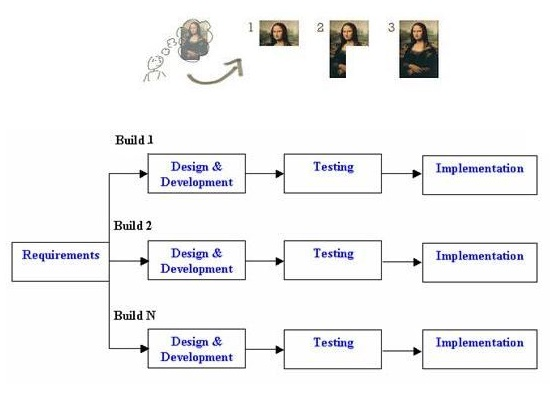
\includegraphics[height=0.35\textheight]{fig01/l_incre}
	\mycaption[Incremental model.]{Incremental model.}
	\label{fig:RHP01}

\end{figure}
\begin{figure}[h]
	\centering
	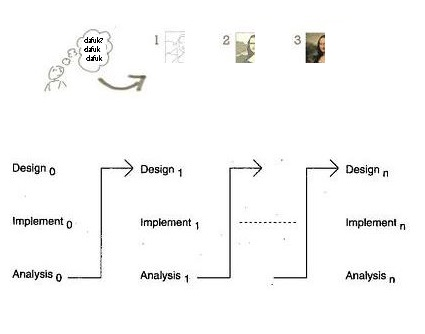
\includegraphics[height=0.35\textheight]{fig01/l_itera}
	\mycaption[Iterative model.]{Iterative model.}
	\label{fig:RHP02}
\end{figure}

Which in unison says, that at every build of incremental model, iteration follows.
\FloatBarrier
\newpage
\subsection{Use Case Model}
\label{subsec:subsec03}

This model describes the user interaction with the system.\\
 A use case is a list of steps, typically defining interactions between a role (known in Unified Modeling Language (UML) as an "actor") and a system, to achieve a goal. The actor can be a human, an external system, or time. \\
In systems engineering, use cases are used at a higher level than within software engineering, often representing missions or stakeholder goals. The detailed requirements may then be captured in Systems Modeling Language (SysML) or as contractual statements.

\begin{figure}[h]
	\centering
	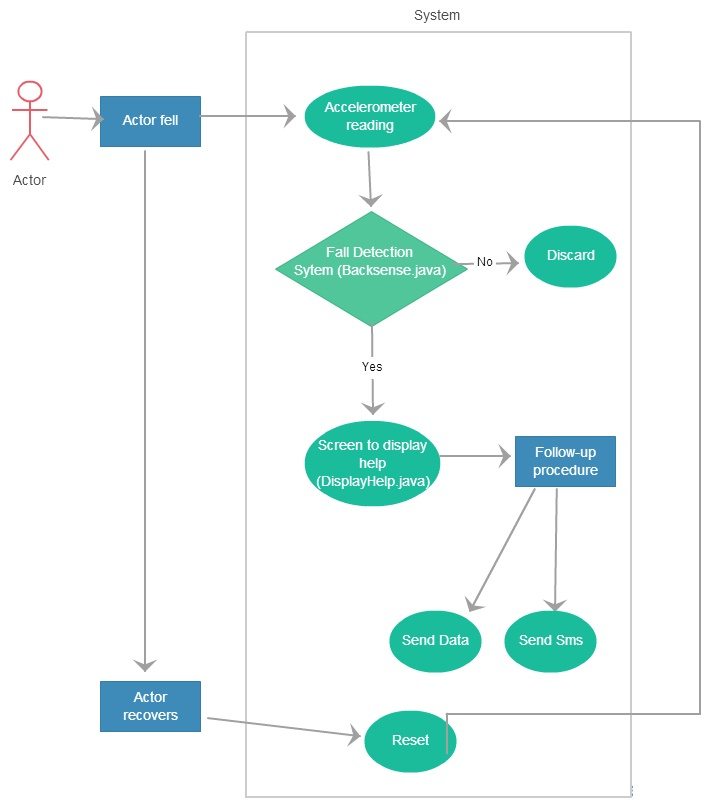
\includegraphics[height=0.61\textheight]{fig01/d_usec}
	\mycaption[Use-case model.]{Use-case model.}
	\label{fig:RHP02}
\end{figure}



\newpage
\section{External Interface Requirement}
\label{sec:sec05}



According to Richard Thayer, ``External interface requirements specify hardware, software, or database elements with which a system or component must interface....''

\subsection{User Interface}
\label{subsec:subsec01}

The `Helpr' has no direct human user interfaces once it is initiated. All human interaction with application is managed by the Android background services and background listeners. \\

Though at the time of installation, a few GUI interaction sessions are there. 

\begin{figure}[h]
	\centering
	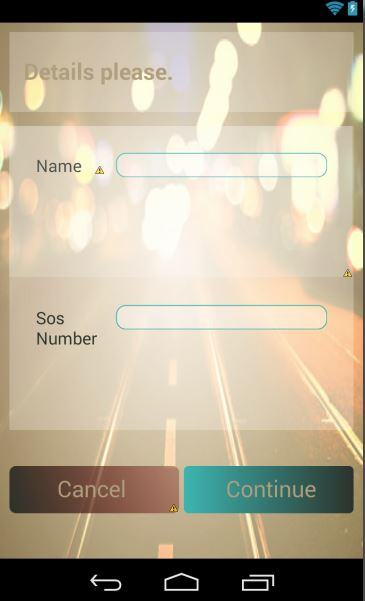
\includegraphics[height=0.35\textheight]{fig01/s_register}
	\mycaption[Screen-shot of Registration page.]{Screen-shot of Registration page.}
	\label{fig:RHP01}

Here the user register itself, by providing a their own name and a contact number, they wish to make the sos-number.
\end{figure}

\begin{figure}[h]
	\centering
	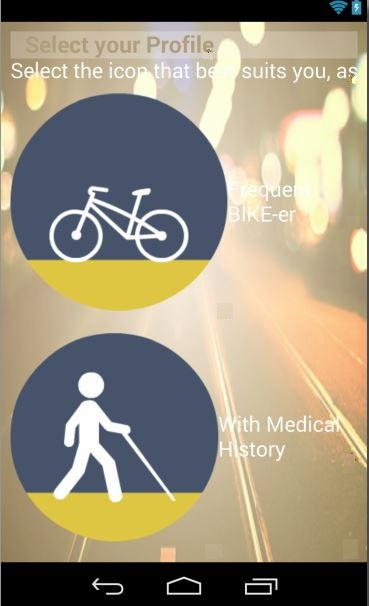
\includegraphics[height=0.35\textheight]{fig01/s_profile}
	\mycaption[Screen-shot of profile selection page.]{Screen-shot of profile selection page.}
	\label{fig:RHP02}

Here the user selects its profile, depending on certain clauses, listed in chapter-5.

\end{figure}
\begin{figure}[h]
	\centering
	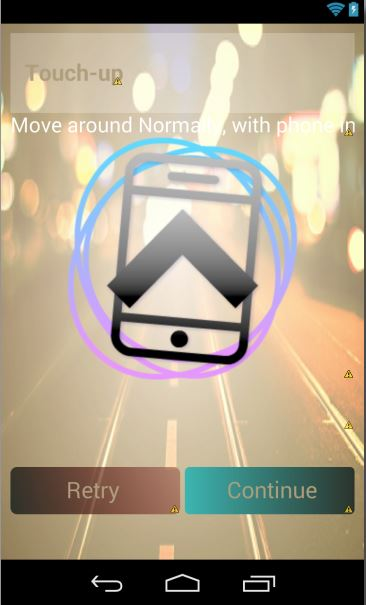
\includegraphics[height=0.35\textheight]{fig01/s_walk}
	\mycaption[Screen-shot of physical activity page.]{Screen-shot of physical activity(walk) page.}
	\label{fig:RHP03}

Here user does a physical interaction session, `a walk with a phone', if it pleases you. So as to gather the base-line of the user's activity.
\end{figure}

\begin{figure}[h]
	\centering
	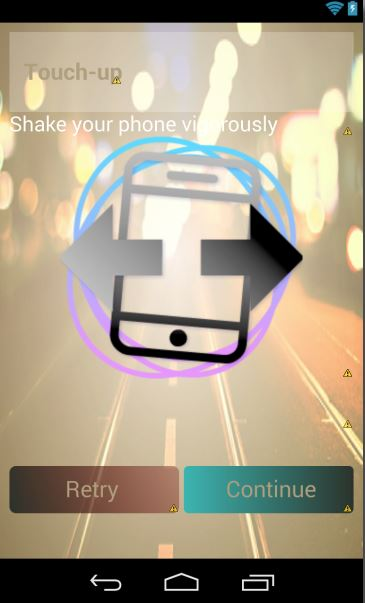
\includegraphics[height=0.35\textheight]{fig01/s_shake}
	\mycaption[Screen-shot of physical activity page..]{Screen-shot of physical activity(shake) page..}
	\label{fig:RHP04}

Here the user shake the phone, so as to have the maxima of the sensors.

\end{figure}
\begin{figure}[h]
	\centering
	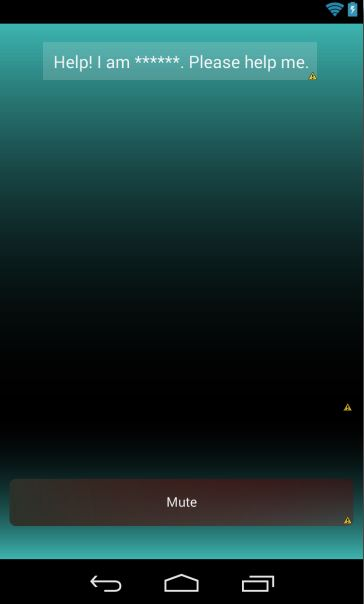
\includegraphics[height=0.35\textheight]{fig01/s_alert}
	\mycaption[Screen-shot of alert.]{Alert page.}
	\label{fig:RHP05}

This is the alert page, which is only visible to user when triggered by human behavior, that the application considers as alarming or not-normal, (falling or getting in an accident).\\
The button at bottom is used to reset the sensor and halt the ongoing process, as listed in chapter-5.
\end{figure}

\FloatBarrier
\subsection{Hardware Interface}
\label{subsec:subsec02}

This flow-chart defines the data flow and interactions that occurs between the hardware and software.\\
We have used:
\begin{figure}[h]
	\centering
	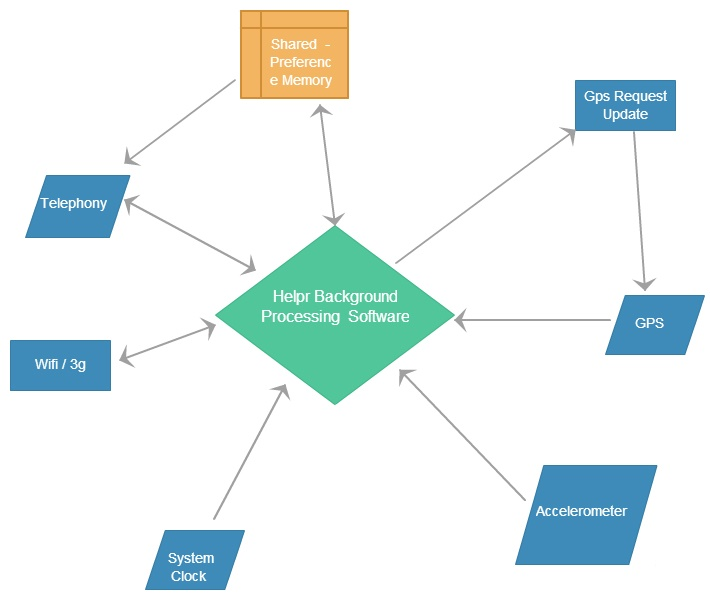
\includegraphics[height=0.41\textheight]{fig01/d_harint}
	\mycaption[Hardware Interaction.]{Hardware Interaction.}
	\label{fig:RHP01}

\begin{description}
\item[$\cdot$ d1] Accelerometer: To track the vector movement.
\item[$\cdot$ d2] GPS: To track the scalar movement on globe.
\item[$\cdot$ d3] SharedPreferece Memory: To store and retrieve data.
\item[$\cdot$ d4] Telephony: To call and receive.
\item[$\cdot$ d5] Network module (cellular/wifi): To send/receive data to server.
\item[$\cdot$ d6] Clock: To have the current system clock.
\end{description}
\end{figure}

\newpage
\subsection{Software Interface}
\label{subsec:subsec03}

This system uses the Android 2.1 or later operating system. Any earlier version is not suppported by this.
In system data is stored and fetched via Sharedpreference memory. As being the data in smaller quantity, it is much faster and light-weight way of fetching it. \\
Global data key are (private):
\begin{description}

\item[$\cdot$ g1] isSplashEnabled : Splash-screen.
\item[$\cdot$ g2] isRegistered : Registered.
\item[$\cdot$ g3] helprname : Name of user.
\item[$\cdot$ g4] helprnumber : Sos number.
\item[$\cdot$ g5] helprlat : latitude of accident.
\item[$\cdot$ g6] helprlon : longitude of accident.
\item[$\cdot$ g7] helpralertactive : Accident occured.
\item[$\cdot$ g8] HelprDataFile : Private keyword to access the data.


\end{description}
On server-side, a general wamp-server like arrangement is provided to store the data.
This data insertion is done by a php web service, created just for the system.


\subsection{Communication Interface}
\label{subsec:subsec04}
This system currently uses two types of communication, \\
SMS : Here the message is sent to the sos number in the following format.\\
\begin{align} 
Help!  I  am  \textbf{\textit{user-name}}.  I  need  your  help.  I  am  at   (approx) \\ Lat: \textbf{\textit{latitude}} \\ Long: \textbf{\textit{longitude}}  \\ Come  get  me!
\end{align}

\newpage
INTERENT : a simple http-post is sent, in `AsyncTask'. with name, phoneNo, lat, long, date.\\

\begin{figure}[h] 
\FloatBarrier
	\centering
	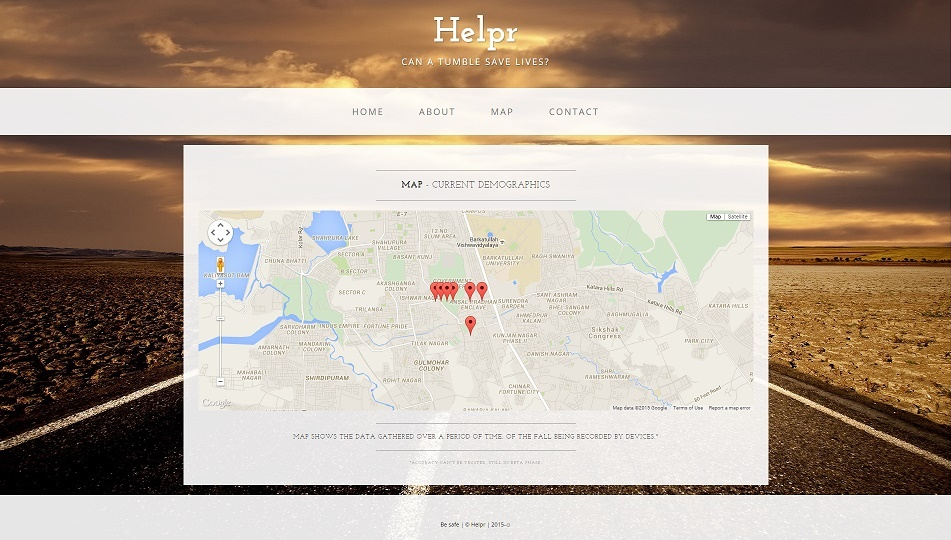
\includegraphics[height=0.47\textheight]{fig01/web}
	\mycaption[Screen-shot of web page.]{The web page.}
	\label{fig:RHP05}

\end{figure}
Map shows the data gathered over a period of time, of the fall being recorded by devices.* \\
The web page shown here, is hosted by the name of  \underline{\textbf{ \textit{www.helpr.cf}}} . All future updates and upgrades will be showcased from here.\\
\vfill
*accuracy can't be trusted, still in beta phase.


%\clearpage
\newpage
%
\section{Non-functional Requirement}
\label{sec:sec06}
Non-functional requirement are not straight forward requirement of the system rather it is related to usability( in some way ).\\
In systems engineering and requirements engineering, a non-functional requirement is a requirement that specifies criteria that can be used to judge the operation of a system, rather than specific behaviors. This should be contrasted with functional requirements that define specific behavior or functions. The plan for implementing functional requirements is detailed in the system design. The plan for implementing non-functional requirements is detailed in the system architecture.\\
Broadly, functional requirements define what a system is supposed to do and non-functional requirements define how a system is supposed to be. Functional requirements are usually in the form of``system shall do <requirement>'', an individual action of part of the system, perhaps explicitly in the sense of a mathematical function, a black box description input, output, process and control functional model or IPO Model. In contrast, non-functional requirements are in the form of ``system shall be <requirement>'', an overall property of the system as a whole or of a particular aspect and not a specific function. The systems' overall properties commonly mark the difference between whether the development project has succeeded or failed.\\
(This write-up is solely due to the erratic behavior of latex editor to not leave a blank page)\\
Non-functional requirements are often called qualities of a system. Other terms for non-functional requirements are `constraints', `quality attributes', `quality goals', `quality of service requirements' and `non-behavioral requirements'. Informally these are sometimes called the `ilities', from attributes like stability and portability.\\


\subsection{Performance Requirement}
\label{subsec:subsec01}
Sensors used for the development and deployment of the project is dependent on the machine (Phone). The phone used should provide viable performance, and ability to manage performance in deemed conditions. \\
Any fault generated is considered as hardware fault, and should be credited as hardware incompatibility issue, with partial software dependency issue.


\subsection{Availability Requirement}
\label{subsec:subsec02}

This application used background services and listener which are active through the life-cycle of a phone. 
Also, allowing certain features could drain the battery life of the system with quite a large amount. Power back-up at ease is advised. However provision to stop the optional detection method is there for the user.

\subsection{Reliability}
\label{subsec:subsec03}
This means the extent to which the application performs with required precision. This again is dependent of hardware; both of phone, and human interaction. \\
False result may occur, when the events are reconstructed.